\documentclass[12pt,a4paper]{article}
\usepackage{fullpage}
\usepackage[margin=2cm]{geometry}
\usepackage{amsmath}
\usepackage{subfig}
\usepackage{graphicx}
\usepackage[justification=centering]{caption}
\usepackage{enumitem}
\usepackage{multirow}
\usepackage{color}

\begin{document}
\title{Landmarks prediction on Beetle anatomical by applying Convolutional Neural Network }
\author{LE Van Linh}
\date{\today}
\maketitle
\begin{abstract}
	In morphometric studies, landmarks are regarded as one of important properties to analyze the object's shape. Especially in biology, collecting complete landmarks give us the information of the oganism. From that, the biologists can study the complex interactions between evolution of the oganism and environment factors. In the context of this study, we focus on one of the most common insect of North-Western France, Carabidae (Beetle). Landmarking manually will be a time-consuming process. In order to investigate the posibility of automatic identify the landmarks on Beetles, we propose a convolutional neural network (CNN) to predict the landmarks on the parts of Beetle: pronotum, head, and body. The proposed model will witnessed on the datasets includes $293$ images (for each part) in different sizes. The experiments will be done in two directions: training the model from scratch and using fine-tuning. During the experiments, the coordinates of automatic landmarks will be evaluated by comparing with the manual coordinates, which are given by the biologists.
\end{abstract}
\section{Introduction}
Morphometric landmarks are important features in biological investigations. They are using to analyze the shape of the organisms. Depending on the organisms, the number of landmarks on their shapes is different. When we consider the position of the landmarks with the shape, most of landmarks are located on the edges, for example, the landmarks on wings of Drosophila fly \cite{.}. Besides, we can also see the landmarks which stayed inside the anatomical part, i.e, landmarks on pinna of human ears \cite{.}. Currently, the landmarks are set manually by the biologsits. However, landmarking manually will be a time-consuming process and difficult to pre-process. Consequently, a process that proposed automatically the coordinates of landmarks could be interested.

In image processing, segmentation is a most often step of the methods. In some cases, the object of interest is easy to extract and can be analyzed with the help of a lot of very well-known image analysis procedures. The result of segmentation step is very useful for many purposes. Depending on purpose of the applications, the object can be segmented or un-segmented before continuing the futher steps. Landmarks setting is no different. In a previous study \cite{.}, we have analyzed two parts of beetle: left and right mandibles. These parts are easy to segment. In that work, we have applied a set of algorithms based on segmentation, image alignment and SIFT \cite{.} to detect the landmarks on mandibles. 

Unfortunately, the images of other parts are not simply as the mandibles. Besides the main objects, we have also the different parts, i.e, we have a part of head and the legs in pronotum images. The image becomes very noisy. If we would like to segment the object as traditional processes, the process may have consumed a lot of time and difficult to choose a proper method. This is the reason that we turn the landmarking problem on some parts of beetle (i.e, pronotum, head, and body) to a way of analyzing images without the segmentation step. 

As the beetles have not been dissected, their anatomical parts have not been set apart. So image segmentation of each part, as they are still attached to the whole specimen, is problematic and has been given up. Coordinates of manual landmarks for each part have been provided and are considered as the ground truth to evaluate the predicted ones by our methods. Fig.\ref{figintro} shows the parts of beeltes and their manual landmarks what we are looking for. 

\begin{figure}[h!]
\centering
\subfloat{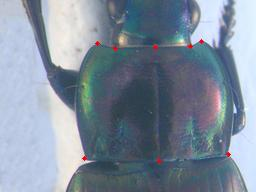
\includegraphics[scale=0.7]{./images/fpronotum}}~~
\subfloat{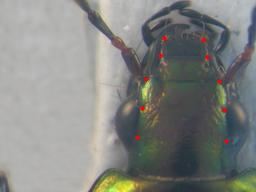
\includegraphics[scale=0.7]{./images/ftete}}~~
\subfloat{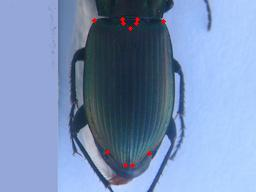
\includegraphics[scale=0.7]{./images/felytre}}
\caption{The dataset images with their manual landmarks.\\
		 \textit{From left to right}: pronotum, head, and body}
\label{figintro}
\end{figure}

To achieve the landmarks prediction, we have proposed a CNN model \cite{.} by using Lasagne library \cite{.}. In the first evaluation, the proposed model has been trained from scratch on the dataset of each part. In the second step, the evaluation has been modified to use a fine-tuning \cite{.} stage.

Our contributions in this study are as follows: In the next section, we present the related works about automatic estimation landmarks on 2D images. The architecture of proposed network will be presented at section \ref{}. In section \ref{.}, we describe the process to augment the dataset. All the experiments of our model will be shown in section \ref{.}. It includes the results to evaluate the model and comparison between two working strategy on neural networks.

\section{Related works}
In geometric morphometry, landmarks (or points of interest) are important features to describe a shape. Depending on the difficulty to segment the objects inside the images, setting automatic landmarks can rely on different methods. When segmentation can be applied, Lowe et al. \cite{.} have proposed a method to identify the key points in the 2D image. From the detected key points, the method is able to match two images. Palaniswamy et al. \cite{.} have applied probabilistic Hough Transform to automatically estimate the landmarks in images
of Drosophila wings. In a previous study \cite{.}, we have extended
Palaniswamy’s method to detect landmarks automatically on
beetles mandibles with good results. Unfortunately, when the
segmentation is not precise, we have observed that the results
are getting worse. This is why we have turned our work on
Deep Learning algorithms in order to find a suitable solution to
predict the landmarks without any segmentation step.

Deep Learning models are coming from machine learning theory. They have been introduced in the middle of previous century for artificial intelligence applications but they encounter
several problems to take real-world cases. More recently, the
improvement of computing capacities, both in memory size
and computing time with GPU programming has opened new
perspective for Deep Learning. Many deep learning architectures have been proposed to solve the problems of classification \cite{.}, image recognition \cite{.}, speech recognition \cite{.} and language translation \cite{.}. To implement
the algorithms, many frameworks have been built such as Caffe
\cite{.}, Theano \cite{.}, Tensorflow \cite{.},.... These frameworks help
the users to design their application by re-using already proposed network architectures. In image analysis domain, Deep
Learning, specifically with CNN, can be used to predict the key
points in an image. Yi Sun et al. \cite{.} have proposed a cascaded
convolutional network to predict the key points on the human
face. Zhang et al. \cite{.} optimize facial landmarks detection
with a set of related tasks such as head pose estimation, age
estimation, ...Cintas et al. \cite{.} have introduced a network to
predict the landmarks on human ear images to characterize ear
shape for biometric analysis. In the same way, we have applied CNN computing to predict the landmarks on beetles anatomical parts. The predicted landmarks will be found in two strategies: training the model from scratch and applying a fine-tuning process.
\section{Dataset}
The data includes images in three sets of the beetle: pronotum, body, and head (Fig.\ref{figdata}). Each dataset includes 293 color images which are taken with the same camera in the same
condition with a resolution of $3264 \times 2448$. Each image has
the manual landmarks setting by biologists, i.e, pronotum has $8$
manual landmarks. For each dataset, the images are randomly divided into two subsets: training and validation (called training set) include 260 images, and the testing set has 33 images.

One of the main characteristics of CNN is that it must use
a huge number of data and one can consider that only several
hundreds of images is not enough to feed a CNN. Moreover,
working with small dataset can push us again to the popular problem of overfitting. A way to enlarge the dataset size
has to be considered. In image processing, we usually apply
transform procedures (translation, rotation) to generate a new
image. Unluckily the methods to compute features through a
CNN most often are translation and rotation independent. So, we have used another method to augment dataset from the down-sampling images. 

\begin{figure}[h!]
	\centering
	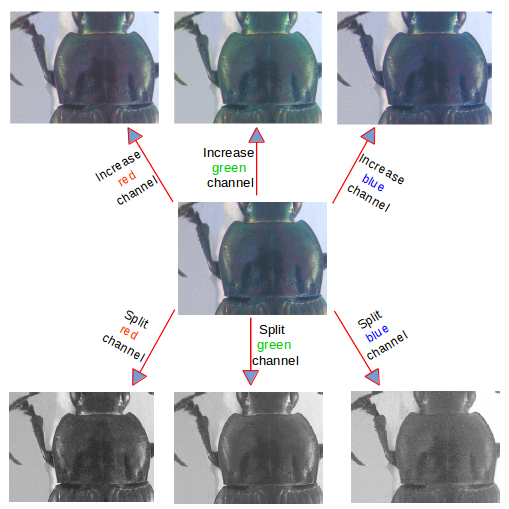
\includegraphics[scale=0.6]{images/cnn_newdatasize/data_aug}
	\caption{An example of augmentation data. From an original image, six augmented version have generated.}
	\label{figdataaug}
\end{figure}

A first procedure has been applied to change the value of
each color channel in the original image. According to that,
a constant is added to one of the RGB channels each time it
is used for training. Each constant is sampled in a uniform
distribution $\in [1,N] $ to obtain a new value caped at $255$. For
example, we can add a constant $c = 10$ to the red channel of
all images in order to generate new images. This operation can
be done for the three color channels. The second procedure separates the channels of RGB into three gray-scale images. As the network works on single channel images we are able to generate six versions of the same image, the total number of images used to train and to validate is
$260 \times 7 = 1820$ images (six versions and original image). This
has been an efficient way to proceed to the dataset expansion. Fig.\ref{figdataaug} presents two strategies that we used to augment the data.

To have obtained the datasets in different sizes of images, we have applied different methods to down-sampling from the original images (see section \ref{}). In the context of this study, we have considered the images in two different resolutions: $256 \times 192$ and $96 \times 96$. Of course, the coordinates of manual landmarks have been also scaled to fit with the new resolutions. In the first considered resolutions ($256 \times 192$), we have simplied down-sampling from the original resolution. While, in the second considered resolution ($96 \times 96$), the original images have been cropped from the left to obtain a new resolution of $2448 \times 2448$. Then, the cropped images have been down-sampled to the target resolution.

\section{The model}
The model, what we used to predict the landmarks, receives an image of $1 \times 256 \times 192$ as the input. The network was constructed from $3$ \textit{``elementary block"} following by $3$ full-connected layers. An elementary block is defined as a sequence of convolution $(C_i)$, pooling $(P_i)$ and dropout $(D_i)$ layers. The parameters for each layers are as below, the list of values follows the order of elementary blocks:
\begin{itemize}[nosep,label=\footnotesize$\bullet$]
	\item CONV layres:
	\begin{itemize}[nosep]
		\item Number of filters: 32, 64 and 128,
		\item Kernel filters size: $(3 \times 3), (2 \times 2)$, and $(2 \times 2)$
		\item Stride values: $1,1,1$
		\item No padding is used for CONV layers
	\end{itemize}
	\item POOL layers:
	\begin{itemize}[nosep]
		\item Kernel filters size: $(2 \times 2), (2 \times 2)$, and $(2 \times 2)$
		\item Stride values: $2,2,2$
		\item No padding is used for CONV layers
	\end{itemize}
	\item DROP layers:
	\begin{itemize}
		\item Propabilities: $0.1, 0.2$ and $0.3$.
	\end{itemize}
\end{itemize}

\begin{figure*}[h]
\centering
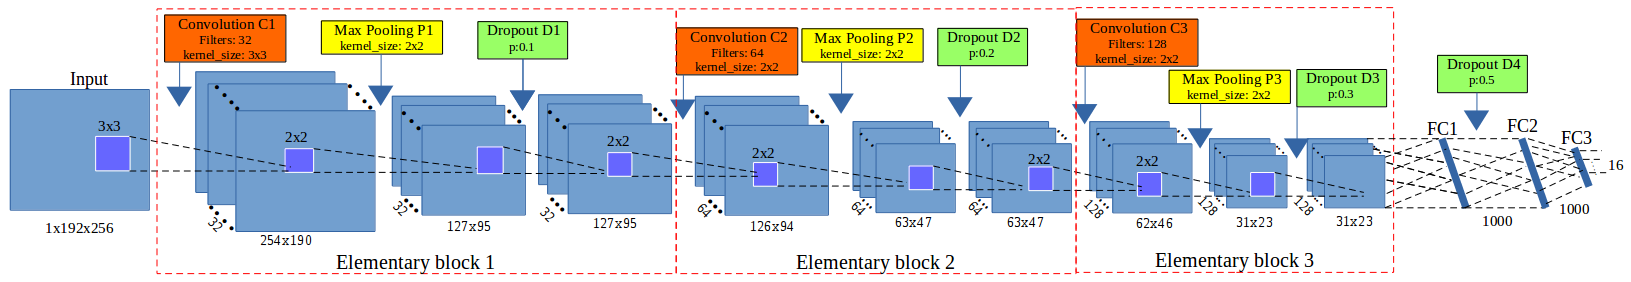
\includegraphics[scale=0.32]{images/cnn_newdatasize/arch_model}
\caption{{\small{Network architecture using $3$ \textit{elementary blocks}.
  Convolution
  layer in red, pooling in yellow and dropout in green color.}}} 
\label{cnnnetwork2}
\end{figure*}
In the last full-connected layers (FC), the parameters are: FC1
output: $1000$, FC2 output: $1000$, FC3 output: $16$. As usual, a
dropout layer is inserted between FC1 ond FC2 with a probability equal to $0.5$. Fig.\ref{cnnnetwork2} illustrate the order of the layers in the network.

The parameters of CNN are shown in Table.\ref{model2parameters}.
\begin{table}[h!]
	\centering
	\begin{tabular}{l l l}
	Parameter & Initial value & End value \\ \hline
	Epochs & 10000 &  \\ \hline
	Training batch size & 128 & \\ \hline
	Testing batch size & 128 & \\ \hline
	Learning rate & 0.03 & 0.0001 \\ \hline
	Momentum & 0.9 & 0.9999 \\ \hline
	\end{tabular}
	\caption{The network parameters in proposed model}
	\label{model2parameters}
\end{table}
\section{Experiments}
The model has been experimented on two resolution datasets: $256 \times 192$ and $96 \times 96$. For each resolution dataset, the model was evaluated in two strategies: training from scratch and fine-tuning. In each evaluation, cross-validation technique to select the training and the testing data. From that, we able to have the predicted landmarks on all images.

The dataset was trained on the model with $10000$ epochs\footnote{An epoch is a single pass through the full training set}. During training, the images are randomly divided into training set and validation set followed the ratio $6:4$. The learning rate began at $0.03$ and decreased to $0.00001$ during training. In vice versa, the momentum started at $0.9$ and increasing to $0.999$ at the end of the training process. 

To evaluate the prediction, the distance between predicted and manual landmarks have been computed in all images. Then, the average distance and standard deviation (SD) have been calculated on each landmark. Following sub-sections describe the average distance and SD of each dataset in each part of beetle.
\subsection{Experiment on the first resolution dataset ($256 \times 192$) }
	\begin{table}[htbp]
		\centering
		\begin{tabular}{ | c | c | c | c | c | }
			\hline
	
			\multicolumn{1}{|c|}{\multirow{2}{*}{Landmarks}} & \multicolumn{2}{c|}{From scratch} &  \multicolumn{2}{c|}{With fine-tuning}  \\ \cline{2-5}
	 & Average & SD & Average & SD \  \\ \hline
			\color{green}{\textbf{LM1}} & \color{green}{\textbf{4.002}} & \color{green}{\textbf{2.5732}} & \color{green}{\textbf{2.486}} & \color{green}{\textbf{1.5448}} \\ \hline
			LM2 & 4.4831 & 2.7583 & 2.7198 & 1.7822 \\ \hline
			LM3 & 4.2959 & 2.7067 & 2.6523 & 1.8386 \\ \hline
			LM4 & 4.3865 & 3.0563 & 2.7709 & 1.9483 \\ \hline
			LM5 & 4.2925 & 2.9086 & 2.4872 & 1.6235 \\ \hline
			\color{red}{\textbf{LM6}} & \color{red}{\textbf{5.3631}} & \color{red}{\textbf{3.4234}} & \color{red}{\textbf{3.0492}} & \color{red}{\textbf{1.991}} \\ \hline
			LM7 & 4.636 & 2.8426 & 2.6836 & 1.7781 \\ \hline
			LM8 & 4.9363 & 3.0801 & 2.8709 & 1.9662 \\ \hline
		\end{tabular}
		\label{tbl1}
		\caption{The average distance and standard deviation on pronotum images}
	\end{table}

	\begin{table}[htbp]
		\centering
		\begin{tabular}{ | c | c | c | c | c | }
			\hline
	
			\multicolumn{1}{|c|}{\multirow{2}{*}{Landmarks}} & \multicolumn{2}{c|}{From scratch} &  \multicolumn{2}{c|}{With fine-tuning}  \\ \cline{2-5}
	 & Average & SD & Average & SD \  \\ \hline
			\color{green}{\textbf{LM1}} & \color{green}{\textbf{3.87}} & \color{green}{\textbf{2.5732}} & \color{green}{\textbf{2.34}} & \color{green}{\textbf{3.11}} \\ \hline
			LM2 & 3.97 & 2.7583 & 2.27 & 3.15 \\ \hline
			LM3 & 3.92 & 2.7067 & 2.27 & 2.96 \\ \hline
			LM4 & 3.87 & 3.0563 & 2.25 & 3.26 \\ \hline
			LM5 & 4.02 & 2.9086 & 2.27 & 3.28 \\ \hline
			\color{red}{\textbf{LM6}} & \color{red}{\textbf{4.84}} & \color{red}{\textbf{3.4234}} & \color{red}{\textbf{3.14}} & \color{red}{\textbf{3.47}} \\ \hline
			LM7 & 5.21 & 2.8426 & 3.14 & 3.40 \\ \hline
			LM8 & 5.47 & 3.0801 & 3.29 & 3.36 \\ \hline
			LM9 & 5.27 & 3.0801 & 3.42 & 3.09 \\ \hline
			LM10 & 4.07 & 3.0801 & 2.49 & 3.05 \\ \hline
			LM11 & 3.99 & 3.0801 & 2.30 & 3.06 \\ \hline						
		\end{tabular}
		\label{tbl2}
		\caption{The average distance and standard deviation on body (elytra) images}
	\end{table}

	\begin{table}[htbp]
		\centering
		\begin{tabular}{ | c | c | c | c | c | }
			\hline
	
			\multicolumn{1}{|c|}{\multirow{2}{*}{Landmarks}} & \multicolumn{2}{c|}{From scratch} &  \multicolumn{2}{c|}{With fine-tuning}  \\ \cline{2-5}
	 & Average & SD & Average & SD \  \\ \hline
			\color{green}{\textbf{LM1}} & \color{green}{\textbf{5.53}} & \color{green}{\textbf{2.5732}} & \color{green}{\textbf{3.03}} & \color{green}{\textbf{1.89}} \\ \hline
			LM2 & 5.16 & 2.7583 & 2.94 & 1.97 \\ \hline
			LM3 & 5.38 & 2.7067 & 2.96 & 1.81 \\ \hline
			LM4 & 5.03 & 3.0563 & 2.88 & 1.92 \\ \hline
			LM5 & 4.84 & 2.9086 & 2.76 & 1.75 \\ \hline
			\color{red}{\textbf{LM6}} & \color{red}{\textbf{4.45}} & \color{red}{\textbf{3.4234}} & \color{red}{\textbf{2.67}} & \color{red}{\textbf{2.02}} \\ \hline
			LM7 & 4.79 & 2.8426 & 2.29 & 1.64 \\ \hline
			LM8 & 4.53 & 3.0801 & 2.20 & 1.54 \\ \hline
			LM9 & 5.14 & 3.0801 & 2.57 & 1.60 \\ \hline
			LM10 & 5.06 & 3.0801 & 2.44 & 1.53 \\ \hline
		\end{tabular}
		\label{tbl3}
		\caption{The average distance and standard deviation on head images}
	\end{table}

Table. \ref{tbl1}, \ref{tbl2}, and \ref{tbl3} show the comparation on average distances and standard deviations on protum, body, and head part, respectively. The results show that the average distance have been improved with using fine-tuning. Besides, we do not see the significant difference of the fine-tuning processes (with and without freezing some layers).
\subsection{Experiment on the second resolution dataset ($96 \times 96$) }
\subsubsection{Pronotum part}
	\begin{table}[htbp]
		\centering
		\begin{tabular}{ | c | c | c | c | c | }
			\hline
	
			\multicolumn{1}{|c|}{\multirow{2}{*}{Landmarks}} & \multicolumn{2}{c|}{From scratch} &  \multicolumn{2}{c|}{With fine-tuning}  \\ \cline{2-5}
	 & Average & SD & Average & SD \  \\ \hline
			\color{green}{\textbf{LM1}} & \color{green}{\textbf{4.002}} & \color{green}{\textbf{2.5732}} & \color{green}{\textbf{2.486}} & \color{green}{\textbf{1.5448}} \\ \hline
			LM2 & 4.4831 & 2.7583 & 2.7198 & 1.7822 \\ \hline
			LM3 & 4.2959 & 2.7067 & 2.6523 & 1.8386 \\ \hline
			LM4 & 4.3865 & 3.0563 & 2.7709 & 1.9483 \\ \hline
			LM5 & 4.2925 & 2.9086 & 2.4872 & 1.6235 \\ \hline
			\color{red}{\textbf{LM6}} & \color{red}{\textbf{5.3631}} & \color{red}{\textbf{3.4234}} & \color{red}{\textbf{3.0492}} & \color{red}{\textbf{1.991}} \\ \hline
			LM7 & 4.636 & 2.8426 & 2.6836 & 1.7781 \\ \hline
			LM8 & 4.9363 & 3.0801 & 2.8709 & 1.9662 \\ \hline
		\end{tabular}
	\end{table}
\subsubsection{Body part}
	\begin{table}[htbp]
		\centering
		\begin{tabular}{ | c | c | c | c | c | }
			\hline
	
			\multicolumn{1}{|c|}{\multirow{2}{*}{Landmarks}} & \multicolumn{2}{c|}{From scratch} &  \multicolumn{2}{c|}{With fine-tuning}  \\ \cline{2-5}
	 & Average & SD & Average & SD \  \\ \hline
			\color{green}{\textbf{LM1}} & \color{green}{\textbf{4.002}} & \color{green}{\textbf{2.5732}} & \color{green}{\textbf{2.486}} & \color{green}{\textbf{1.5448}} \\ \hline
			LM2 & 4.4831 & 2.7583 & 2.7198 & 1.7822 \\ \hline
			LM3 & 4.2959 & 2.7067 & 2.6523 & 1.8386 \\ \hline
			LM4 & 4.3865 & 3.0563 & 2.7709 & 1.9483 \\ \hline
			LM5 & 4.2925 & 2.9086 & 2.4872 & 1.6235 \\ \hline
			\color{red}{\textbf{LM6}} & \color{red}{\textbf{5.3631}} & \color{red}{\textbf{3.4234}} & \color{red}{\textbf{3.0492}} & \color{red}{\textbf{1.991}} \\ \hline
			LM7 & 4.636 & 2.8426 & 2.6836 & 1.7781 \\ \hline
			LM8 & 4.9363 & 3.0801 & 2.8709 & 1.9662 \\ \hline
		\end{tabular}
	\end{table}
\subsubsection{Head}
	\begin{table}[htbp]
		\centering
		\begin{tabular}{ | c | c | c | c | c | }
			\hline
	
			\multicolumn{1}{|c|}{\multirow{2}{*}{Landmarks}} & \multicolumn{2}{c|}{From scratch} &  \multicolumn{2}{c|}{With fine-tuning}  \\ \cline{2-5}
	 & Average & SD & Average & SD \  \\ \hline
			\color{green}{\textbf{LM1}} & \color{green}{\textbf{4.002}} & \color{green}{\textbf{2.5732}} & \color{green}{\textbf{2.486}} & \color{green}{\textbf{1.5448}} \\ \hline
			LM2 & 4.4831 & 2.7583 & 2.7198 & 1.7822 \\ \hline
			LM3 & 4.2959 & 2.7067 & 2.6523 & 1.8386 \\ \hline
			LM4 & 4.3865 & 3.0563 & 2.7709 & 1.9483 \\ \hline
			LM5 & 4.2925 & 2.9086 & 2.4872 & 1.6235 \\ \hline
			\color{red}{\textbf{LM6}} & \color{red}{\textbf{5.3631}} & \color{red}{\textbf{3.4234}} & \color{red}{\textbf{3.0492}} & \color{red}{\textbf{1.991}} \\ \hline
			LM7 & 4.636 & 2.8426 & 2.6836 & 1.7781 \\ \hline
			LM8 & 4.9363 & 3.0801 & 2.8709 & 1.9662 \\ \hline
		\end{tabular}
	\end{table}


\subsection{Training on three parts of beetle}


Fig.\ref{figlossallparts} shows the losses during training process. At the beginning, the validation loss is always higher than the tranining loss, but from the $2000^{}$ epochs, the training loss begins stable while the validation loss continue to decrease. At the end of training, the losses values are $0.00029$ and $0.00009$ for training and validation, respectively.

\begin{figure}[h!]
	\centering
	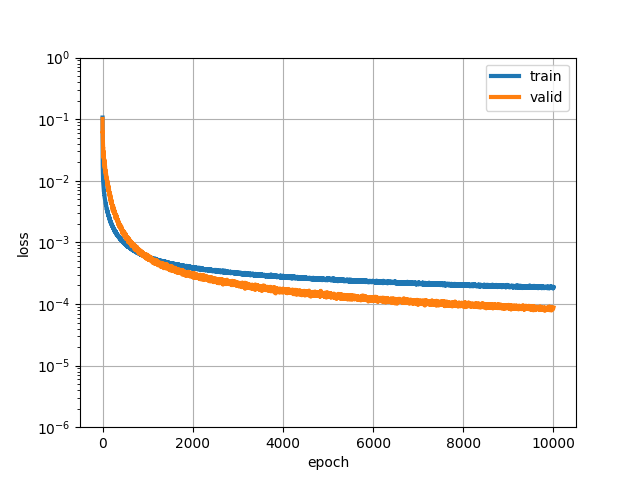
\includegraphics[scale=0.6]{images/all_parts_10000epochs}
	\caption{The losses during training on the images of three parts}
	\label{figlossallparts}
\end{figure}

Fig.\ref{figtestallparts} shows the predicted landmarks on some images in test set.
\begin{figure}[h!]
	\centering
	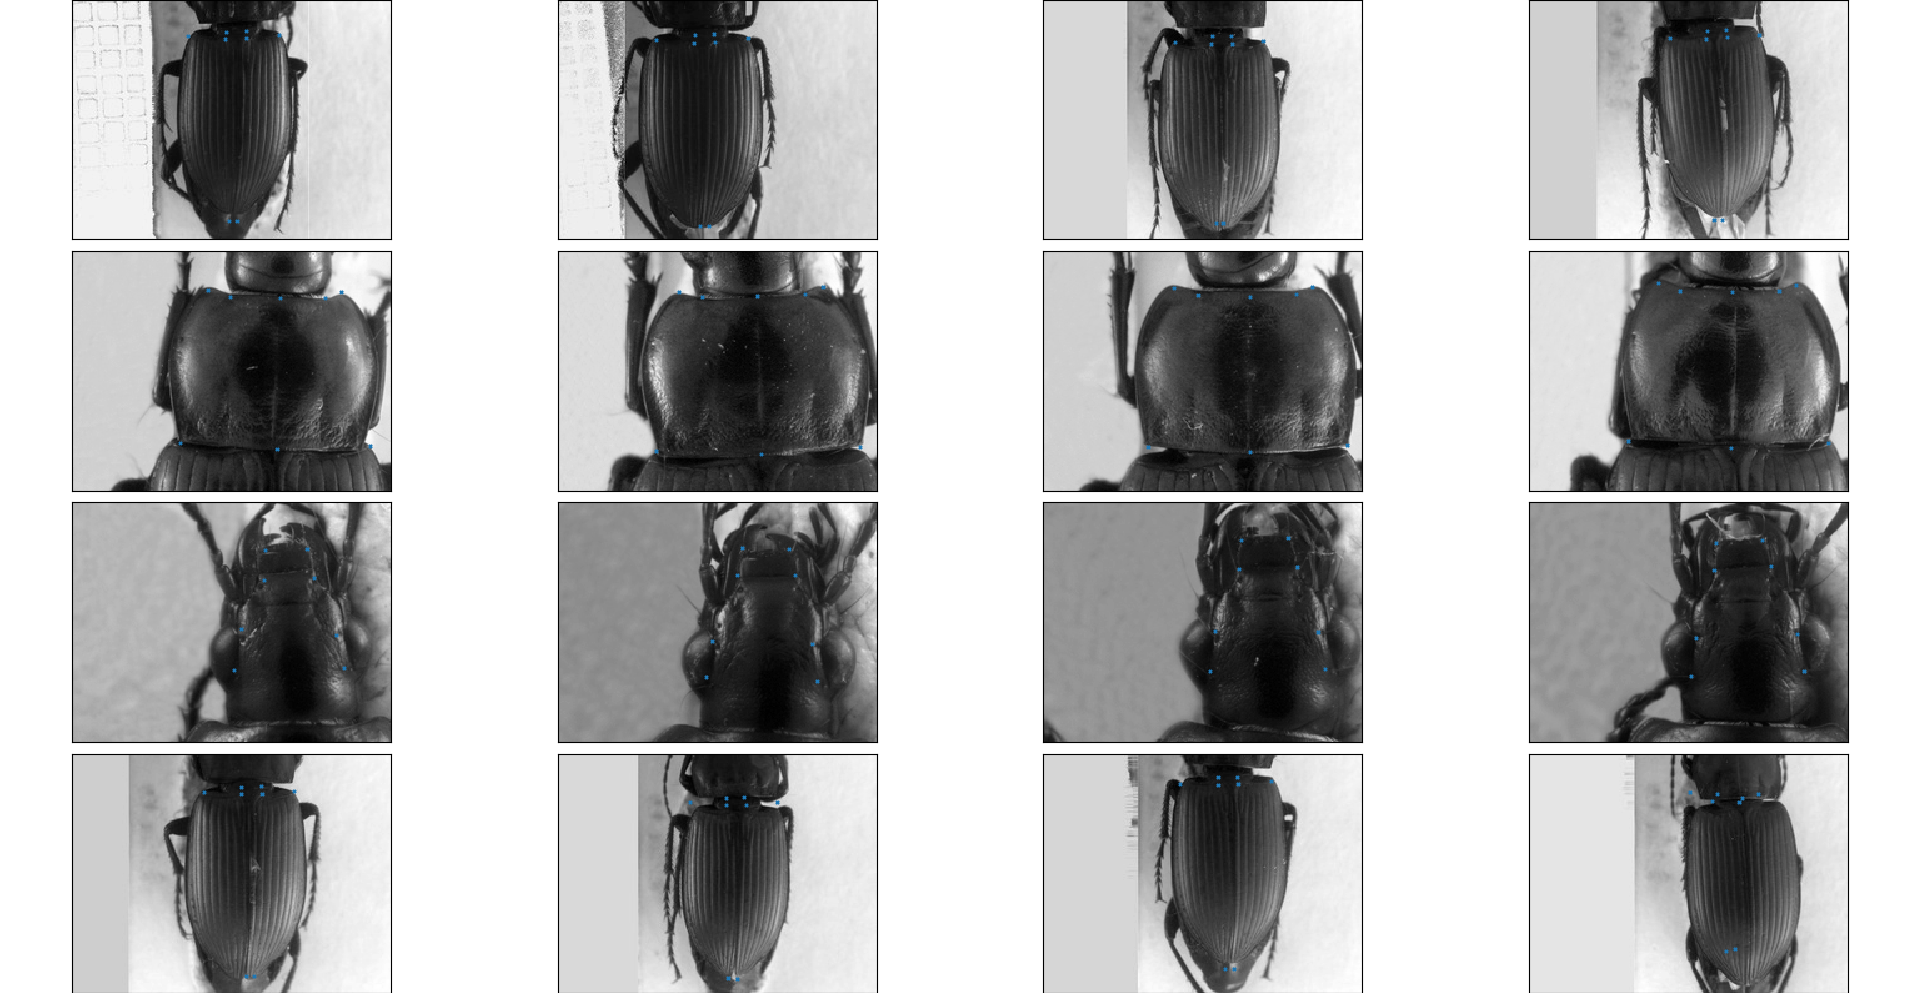
\includegraphics[scale=0.53]{images/all_parts_10000epochs_test}
	\caption{The blue points present for the predicted landmarks on the images in test set}
	\label{figtestallparts}
\end{figure}
\subsection{Fine-tuning on pronotum dataset}
The trained model have been continued to fine-tune \cite{yosinski2014transferable} with pronotum dataset. To get all predicted landmarks for the pronotum images, a scenario to choose the test images is executed. For each round, we have chosen 33 images for the test set, the remaining images have been put to training test. Table.\ref{finetuningloss} shows the losses during fine-tuning on different dataset of pronotum images.

\begin{table}[h!]
	\centering
	\begin{tabular}{l l l}
	Round & Training loss & Validation loss \\ \hline
	1 & 0.00019 & 0.00009  \\ \hline
	2 & 0.00018 & 0.00010 \\ \hline
	3 & 0.00018 & 0.00010 \\ \hline
	4 & 0.00019 & 0.00008 \\ \hline
	5 & 0.00019 & 0.00009 \\ \hline
	6 & 0.00018 & 0.00008 \\ \hline
	7 & 0.00019 & 0.00008 \\ \hline
	8 & 0.00018 & 0.00006 \\ \hline
	9 & 0.00018 & 0.00009 \\ \hline
	\end{tabular}
	\caption{The losses during fine-tuning model}
	\label{finetuningloss}
\end{table}

Fig.\ref{figfintuning} shows an example of the losses during fine-tuning and corresponding predicted landmarks on the test set.

\begin{figure}[h!]
\centering
\subfloat[Training losses and validation loss]{\label{model1loss}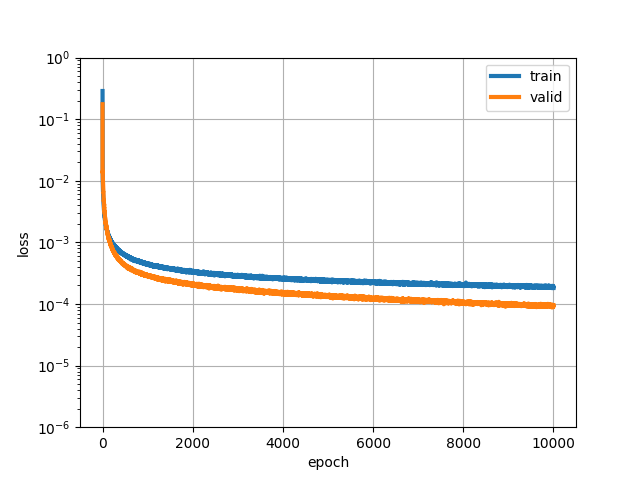
\includegraphics[width=0.3\textwidth]{./images/pronotum_fine_tuning_v11}}~~
\subfloat[A pronotum with predicted landmarks]{\label{model1test}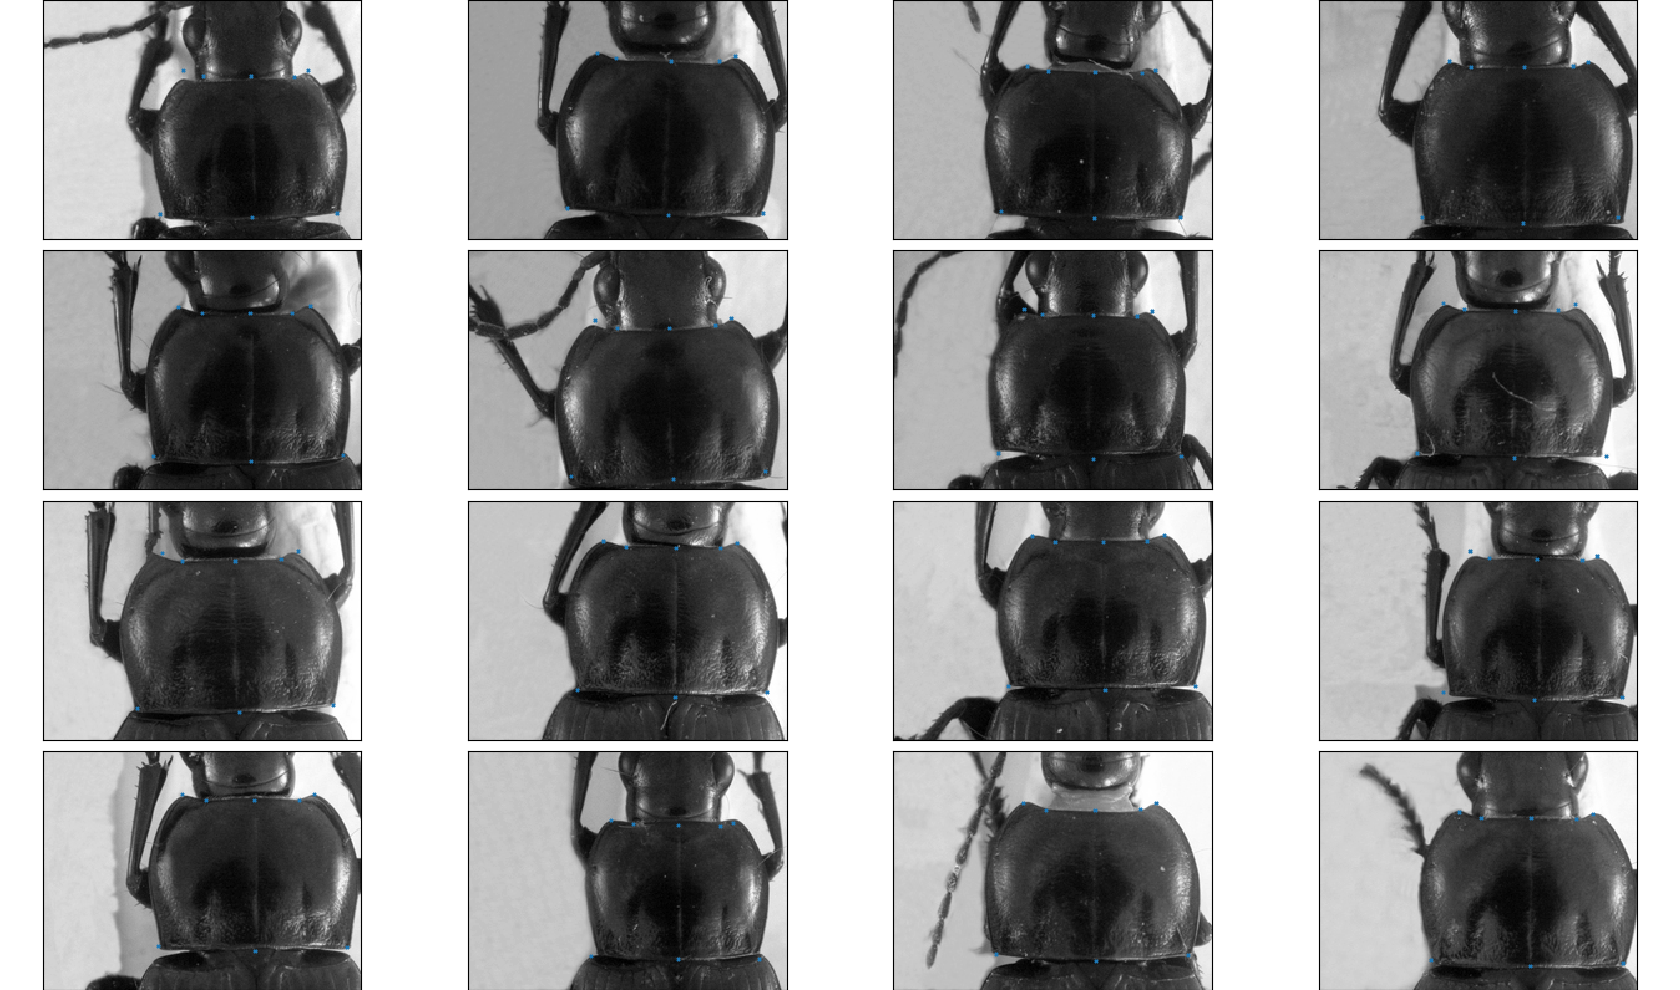
\includegraphics[width=0.7\textwidth]{./images/pronotum_fine_tuning_v11_test}}
\caption{An result example when fine-tuning the trained model on pronotum dataset}
\label{figfintuning}
\end{figure}
After fine-tuning, the predicted landmarks of all images are provided. To evaluate the effects of fine-tuning, we calculated the distance between the predicted landmarks and corresponding manual landmarks. A statistic on the distance of each landmarks is also computed. 

Table.\ref{tab2} shows the average error distance given by each landmark. The values in \textbf{Distance 1} and \textbf{Distance 2} columns present for the average distance of all landmark when the pronotum images were trained from scratch and fine-tuning, respectively. From the Table. \ref{tab2}, the result from fine-tuning is significantly improved ($\sim 38\%$) 
\begin{table}[htbp]
\begin{center}
\begin{tabular}{|c|p{2.5cm}|p{2.5cm}|}
\hline
\textbf{$\#$Landmark} & \textbf{Distance 1} & \textbf{Distance 2} \\ \hline
1 & 4.002 & 2.486  \\ \hline
2 & 4.4831 & 2.720  \\ \hline
3 & 4.2959  & 2.652 \\ \hline
4 & 4.3865  & 2.771 \\ \hline
5 & 4.2925  & 2.487 \\ \hline
6 & 5.3631  & 3.049 \\ \hline
7 & 4.636  & 2.684 \\ \hline
8 & 4.9363  & 2.871 \\ \hline
\end{tabular}
\caption{The average error distance per landmark.}
\label{tab2}
\end{center}
\end{table}

\section{Conclusions}
A CNN model has been trained on a dataset that includes the images of three parts of beetle. The trained model then has been fine-tuned with the pronotum dataset. Comparing the losses when we trained the pronotum from scratch, the losses during fine-tuning has been improved $40\%$ on validation test. Besides, the coordinates of predicted landmarks are also more accuracy than the last result (training from scratch) (Table.\ref{tab2}). From the result, we can see that fine-tuning has affected to the results from CNN. However, the effects still limits in our case. The experiments of the techniques on fine-tuning need to do to reach to the result as we expect.
\bibliographystyle{unsrt}
\bibliography{includes/references}

\end{document}
